\section{Packet Processing Pipeline}

The OpenFlow specifications imply 

% problem - how to simulate many different pipelines
%  - openflow presents many versions
%  - even within a version there is a great degree of optionality allowed
%  - there are non-openflow pipelines that we would like to simulate
% primary value of this section
% - flexible - can emulate a wide variety of OF and non-OF systems
% - 

% the pipeline is like a directed graph 
% - composes of stages (nodes)
%   - stage is like an object with a step method
%   - parametric construction supports a wide range of behaviors
%   - step operates over one or more inputs and returns and output
%   - datatype is a Context
% - control flow connections (directed edges)
%   - data flows from the output of a stage to the input of another stage
%   - when there are more than one input there is implicit queuing in a stage

% there are two types of dynamic scopings
% - context scope
%   - this is the scope of an event the pipeline is processing
%   - lifetime of variables
% - pipeline scope
%   - this is the scope of the pipeline organization
%   - lifetime of variables 

% simulation is composed of ...
% - pipeline
% - packet trace

% terms ::= pipeline | stage | context | lifetime | lifecycle | trace

FlowSim provides a packet processing pipeline that can be configured to emulate
a wide range of differing OpenFlow pipelines an non-OpenFlow packet processing
behaviors.

A pipeline is a collection of stages and control flow edges. Each stage can be
thought of as a function that operates over one or more inputs and returns an 
output. The datatype that flows between stages is called the Context.

A pipeline computes
by moving a generic data structure, called the Context, between 

The pipeline is composed of seven stages: Arrival, Extraction, Choice, 
Selection, Execution, Group, and Egress. Stages are connected together to
form a directed graph

\begin{figure}[h]
  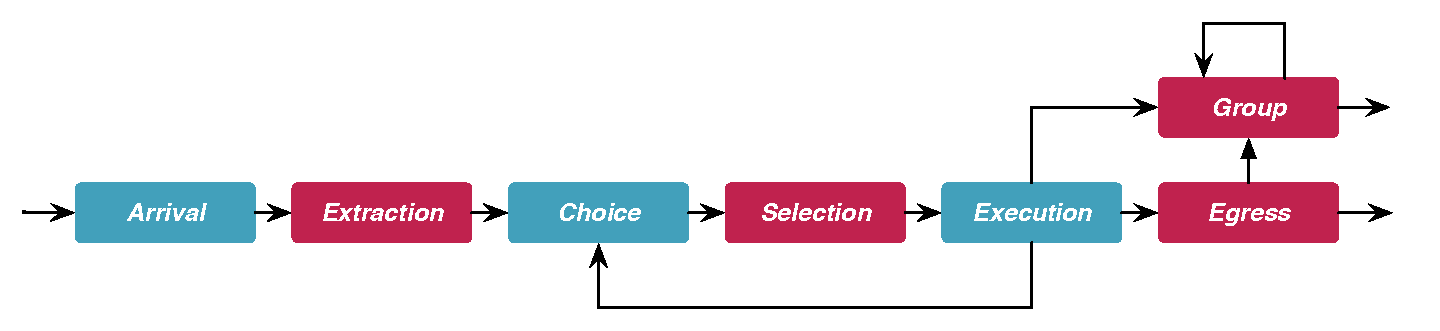
\includegraphics[width=\linewidth]{figures/pipeline.pdf}
  \label{figure:pipeline}
  \caption{FlowSim Switch Pipeline}
\end{figure}

\begin{figure}
  \lstinputlisting{code/context.steve}
  \label{listing:context}
  \caption{Context Datatype}
\end{figure}

\begin{figure}
  \lstinputlisting{code/internal.steve}
  \label{listing:internal}
  \caption{Internal Datatype}
\end{figure}
